\section{Benchmark and Protocol}
\label{sec:benchmark}

\subsection{Corruption taxonomy}

Nine corruptions are grouped into four disaster families: flood
(\cfd{water\_glare}, \cfd{turbidity\_cast}, \cfd{inundation}), wildfire
(\cfd{smoke\_haze}, \cfd{fire\_warm\_tint}), storm (\cfd{rain\_streaks},
\cfd{motion\_blur}, \cfd{low\_light}), and earthquake and post-disaster
(\cfd{dust\_haze}); see Figure~\ref{fig:taxonomy}. Grouping by disaster
family rather than by distortion type is deliberate, so a result reads
as ``this system loses $X$ of its detections in wildfire smoke'' rather
than as a filter name. With three severities each plus the clean
condition, one model on one dataset is measured over 28 conditions, and
the full study over 168.

\subsection{Physical models}

The three haze-family corruptions are built on the Koschmieder
atmospheric scattering model~\cite{koschmieder1924theorie,narasimhan2002vision},
$I = Jt + A(1-t)$, with $J$ the clear-scene radiance, $A$ the
atmospheric light and $t$ the transmission map. \cfd{smoke\_haze} and
\cfd{dust\_haze} differ principally in the chromaticity of $A$, neutral
grey for combustion aerosol against a brown mineral airlight for
suspended particulate, a distinction verified by a unit test on the
red-to-blue channel ratio. Sediment-laden water is not a scattering
process, so the flood family is modelled separately: \cfd{turbidity\_cast}
blends toward a mud chromaticity with contrast compression toward the
scene mean and saturation loss, \cfd{water\_glare} adds thresholded
specular glint cores with a Gaussian bloom halo, and \cfd{inundation}
composites semi-transparent standing water over part of the scene with a
ripple displacement of the submerged content.

\cfd{low\_light} is modelled in the linear photometric
domain~\cite{chen2018dark}. The image is linearised, scaled by a photon
gain, given a twilight blue shift, and returned through the transfer
curve with signal-dependent shot noise and signal-independent read noise
whose relative magnitude grows as light falls. This matters for what the
benchmark measures: the severities are not a gamma darkening but a loss
of photons, so contrast and signal-to-noise degrade together the way
they do on a real sensor at dusk. The three severities apply linear
gains of 0.33, 0.13 and 0.045, which is an exposure loss of roughly 1.6,
2.9 and 4.5 stops, with the read-noise floor rising from 0.010 to 0.028
across the ladder. Severity 3 is therefore late dusk rather than
darkness, which is worth keeping in mind against the results that
follow. \cfd{rain\_streaks} follows the additive
directional-streak model of Garg and Nayar~\cite{garg2007rain}, and
\cfd{motion\_blur} applies a directional kernel scaled to image size.

\subsection{Calibration}

Each corruption declares a measurable image statistic that must move
monotonically across its three severities, verified on a fixed random
20-image subset held constant across all corruptions so that comparisons
are made against identical scene content. Eight of nine pass directly.
\cfd{rain\_streaks} does not: its declared statistic, streak density,
has no closed-form image measure, and the substituted edge-strength
proxy is confounded because added streaks raise measured edge strength
while the veil blur suppresses it. Its severity is instead defined by
monotonically increasing generation parameters (streaks per megapixel,
streak length and veil intensity) and verified by visual audit;
downstream recall degrades in the expected direction regardless,
independent evidence that the corruption intensifies even though this
one proxy does not track it. We report this rather than substituting a
statistic chosen after the fact for passing.

The statistic calibrates each ladder \emph{within} a corruption; it is
not a cross-corruption difficulty normaliser, and two corruptions
matched on the same statistic are not expected to be equally damaging.
\cfd{smoke\_haze} and \cfd{dust\_haze} illustrate this directly: they
reach nearly identical RMS contrast at every severity (0.0475 versus
0.0489 at severity 3) yet differ 6.7-fold in cost
(Table~\ref{tab:spectrum} and Table~\ref{tab:family}), showing detection
difficulty here is not reducible to global contrast reduction alone. We
do not isolate which remaining difference, airlight chromaticity,
transmission-field granularity or added grain, carries the effect, and
flag it as an open question.

\subsection{Determinism and reproducibility}

Pixel-unit parameters are specified per 1000 pixels of the longer image
side and scaled at runtime, so a severity means the same thing across
capture regimes. Corruptions are appearance-only, leaving clean
ground-truth boxes exactly valid. Every stochastic element is seeded
from a SHA-256 stable hash of image identity, corruption, severity and
global seed, independent of platform, so the corrupted benchmark
regenerates bit-identically anywhere. We redistribute no imagery; the
released code and parameters reproduce it from the source datasets,
which preserves both licences and the ability to audit what was applied.

\subsection{Datasets and detectors}

HERIDAL~\cite{bozic2019heridal} is captured at high altitude over
wilderness terrain at $4000 \times 3000$, and its test split holds 101
images with 337 annotated persons. The evaluated SARD~\cite{sambolek2021sard}
copy is a re-export at $640 \times 640$, captured lower with larger
relative object size, and its test split holds 862 images with 1097
persons. The two therefore span the high- and low-altitude capture
regimes, which is what makes the transfer question in
Section~\ref{sec:results} answerable at all.

Both datasets pass through the same tiling pipeline, 1024-pixel tiles at
256-pixel overlap, chosen so the overlap exceeds the largest person box.
On HERIDAL this genuinely tiles each frame into 20; on SARD the source
frames are smaller than the tile, so each passes through as a single
full-frame tile. Running one protocol on both is deliberate, since it
removes an experimenter degree of freedom when comparing capture
regimes, and we state the differing behaviour rather than hiding it.
Predictions are mapped back and evaluated against full-resolution ground
truth after class-agnostic non-maximum suppression.

We fine-tune three architecturally distinct detectors: Faster
R-CNN~\cite{ren2015fasterrcnn} (two-stage CNN),
YOLOv11~\cite{ultralytics2024yolo11} (single-stage CNN) and
RT-DETR~\cite{zhao2024rtdetr} (transformer), one run per model per
dataset, all at 1024-pixel input on a single 8\,GB consumer GPU. The
hardware budget is worth stating because it means the benchmark is
reproducible without cluster access. Training is the standard recipe for
each framework rather than a tuned one, since the object of study is the
evaluation axis and not a new detector.

\subsection{Evaluation protocol}

Thresholds are selected once per model per dataset by maximising F1 on
clean validation data and frozen across all 28 conditions for that
model; corrupted data enters neither training nor threshold selection.
This is the single most consequential protocol choice in the paper. A
threshold retuned per condition would report the best case available to
an oracle, which is not a case a fielded system has access to mid-mission,
and it would hide exactly the failure we find.

All architectures are scored by one evaluator, greedy score-ordered
matching at IoU $\geq 0.5$, so no model is scored by its own framework's
metric. Corruptions are applied to the full frame before tiling, since
haze gradients and flood masks are spatially coherent across a scene and
applying them per tile would introduce seams the physics does not
produce. Degradation is reported relative to each model's own clean
score, since the datasets do not share a difficulty floor. Confidence
intervals are bootstrap percentile over 1000 resamples of the test set
by image~\cite{efron1993bootstrap}, resampling images rather than
instances so that the interval reflects scene-level variability.

\begin{figure}[t]
\centering
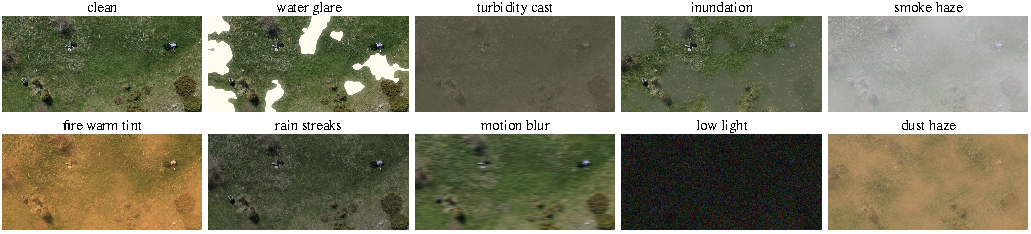
\includegraphics[width=\columnwidth]{figures/taxonomy_s3.pdf}
\caption{The nine corruptions at severity 3 on a cropped HERIDAL frame.
Each models a documented optical signature of a disaster environment
rather than a generic distortion.}
\label{fig:taxonomy}
\end{figure}
